%!TEX root = ../thesis.tex
%*******************************************************************************
%****************************** Sixth Chapter **********************************
%*******************************************************************************
\chapter{Implementation}

\graphicspath{{Chapter6/Figs/Raster/}{Chapter6/Figs/}}

\section{Development Environment and Tools}

\begin{figure}[!ht] 
    \centering    
    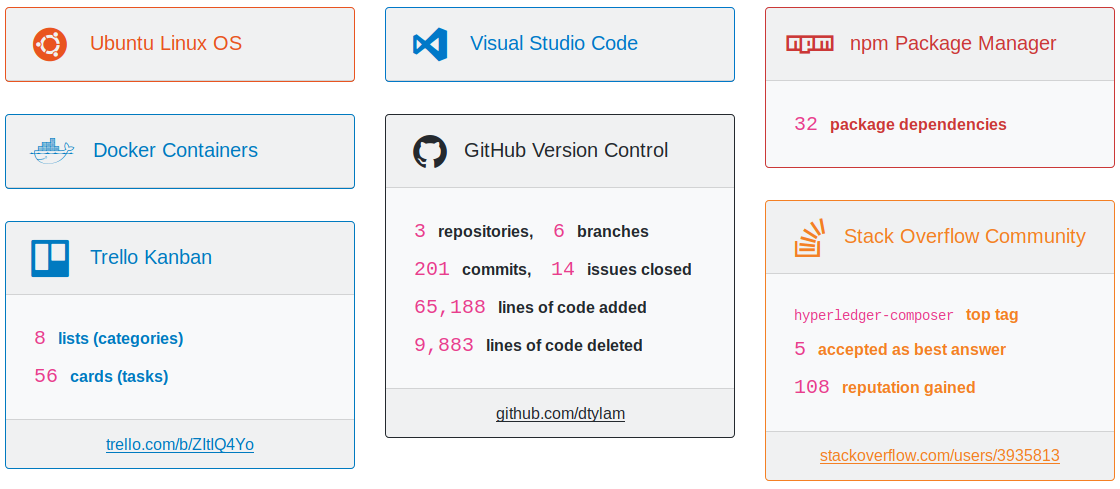
\includegraphics[width=1.0\textwidth]{platform_stats}
    \caption[Development Tools and Usage Statistics]
        {A visual overview of the tools used and their usage statistics if any} 
    \label{fig:platform_stats}
\end{figure}

Specific systems and tools were used to build the demonstrator network and client applications (as in Figure \ref{fig:platform_stats}). 
These choices and their rationale are detailed below:

\underline{Operating System}: The developer's guide for both Hyperledger Composer and Hyperledger Fabric 
recommends using Ubuntu or Mac OS as the host operating system for development. 
Ubuntu is selected for being the free and open source option. The development personal computer, which was originally 
a Windows machine, was set up to dual boot with the latest Ubuntu release.

\underline{Version Control}: A version control system or software keeps track of source code modifications, 
so that developers can compare earlier versions of the code, revert changes, and 
minimise disruptions of mistakes \citep{atlassian2018vcs}. It is essential to medium to large scaled projects.

All work done at the implementation stage was tracked with the version control system Git. 
Git is a distributed version control system, where repositories can be backed up to a remote server, 
such as on the cloud. This is done with GitHub, a git-based version control, code hosting and 
project management service that offers free private repositories to verified students \citep{github2018education}.

\underline{Code Editor}: The Hyperledger Composer framework does not require a dedicated integrated 
development environment and recommends using a text editor. Visual Studio Code, an open source text editor developed 
by Microsoft was chosen as it has a dedicated official syntax checking and beautifying plugin for Hyperledger Composer.

\underline{Community Support}: Hyperledger Composer and Hyperledger Fabric have active communities on Stack Overflow, 
a popular online community forums for developers to discuss coding problems. Throughout the duration of the project, 
it has been a source of solutions to common problems faced and solved by many other users. Towards the end of the project, 
answer contributions were also made.

Several other tools were also used, for example, as previously mentioned in Chapter 3, Trello was used to manage 
feature prioritisation for the agile development process. The use of Docker containers and npm package manager 
will be explained in due course below.

\section{Architecture and Tech Stack}

\begin{figure}[!ht] 
    \centering    
    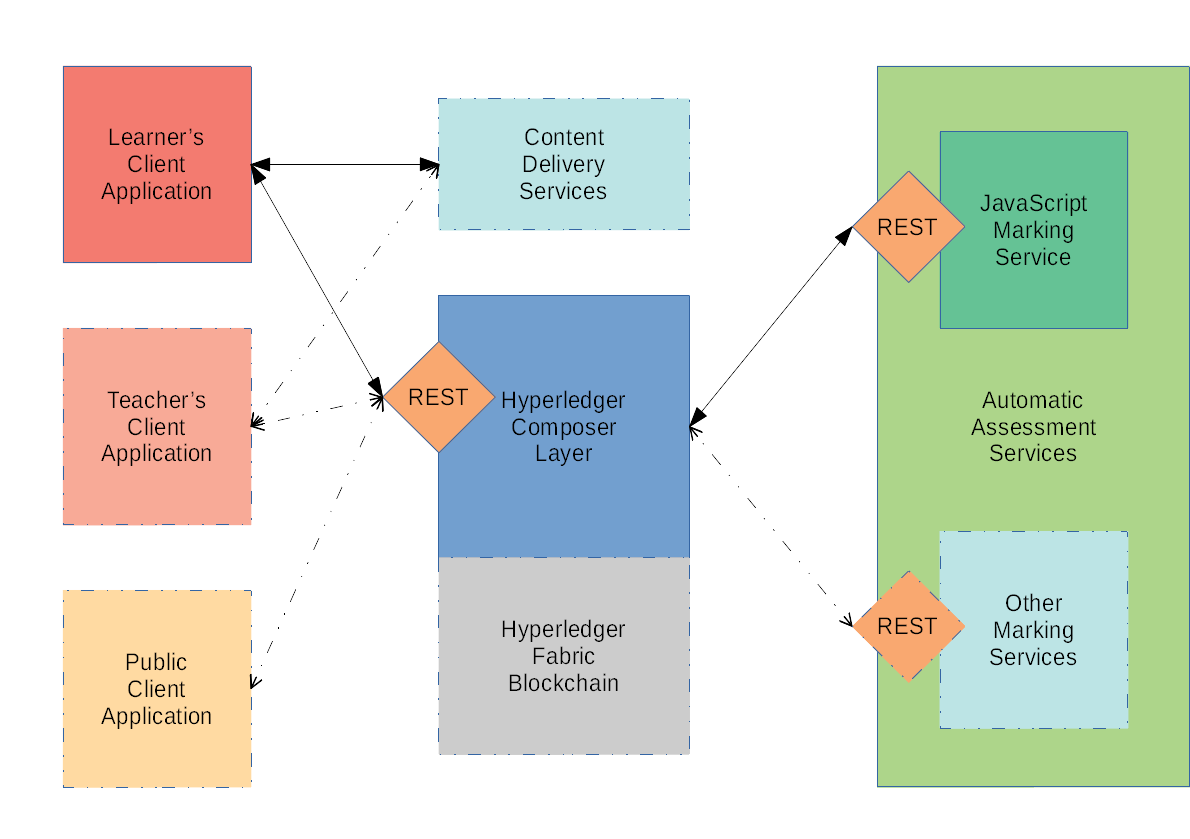
\includegraphics[width=0.9\textwidth]{architecture}
    \caption[Demonstrator Component Architecture]
        {Component architecture overview for the demonstrator system built (dashed lines components were not built)}
    \label{fig:architecture}
\end{figure}

The microservices architecture pattern is used to design the demonstrator system. Microservices is a pattern proposed by 
\citet{richardson2018ms} that structures a system as a set of loosely coupled, collaborating services, partitioned so that 
each service corresponds to a business capability.

In the demonstrator system (as in Figure \ref{fig:architecture}), this is exemplified by the separation of teacher and student applications, 
the separation of content delivery and student records (blockchain), and the separation of different automatic marking services.
They communicate through RESTful web protocols (HTTP and JSON). 
This also enables the use of different technologies, separate testing and deployment for each component.

Figure \ref{fig:techstack} shows an alternate overview of the demonstrator system with its technology stack. 
These main software packages are described further below.

\begin{figure}[!ht] 
    \centering    
    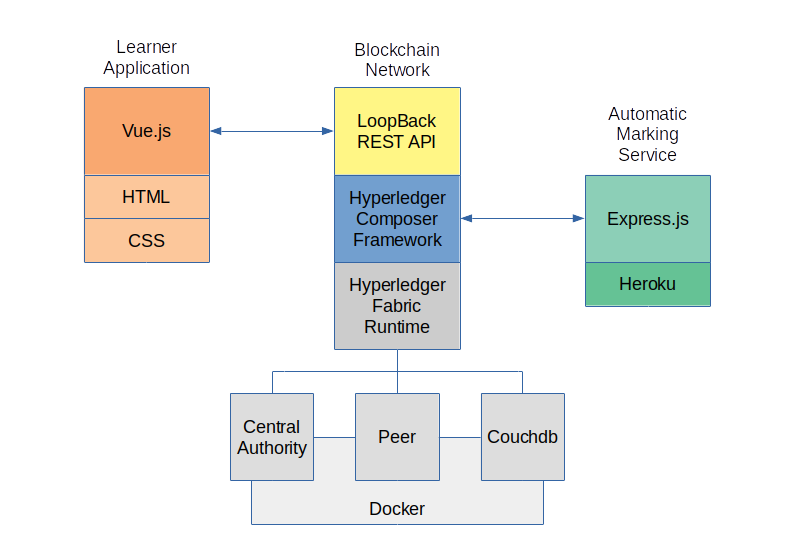
\includegraphics[width=0.85\textwidth]{techstack}
    \caption[Demonstrator Technology Stack]
        {Technology Stack overview for the demonstrator system built}
    \label{fig:techstack}
\end{figure} 

\subsection{Client Applications}

The client applications for learners and teachers has to be highly dynamic (non-static) web applications, 
with the JavaScript scripting language facilitating most of the user interactions.

Vue.js is a JavaScript-based framework for developing web interfaces. Vue.js was chosen over other 
popular frameworks such as React.js and Angular.js because it is focused on the view layer and is much 
simpler and faster to learn. The Node.js JavaScript runtime is used to run the Vue.js applications. The npm package manager 
is used to install and manage the packages used. See more details such as version numbers in Appendix B.1.

\subsection{Blockchain Network}

Hyperledger Composer deploys to Hyperledger Fabric, which runs on Docker.
Docker is a containerisation platform used to develop distributed systems. 
A container is a lightweight, stand-alone package of a piece of software that includes everything 
needed to run it from code and tools to system settings. 

Docker can emulate multiple servers and run them separately on one development machine. 
This provides the peers network needed to host the distributed ledger required for the 
Hyperledger Fabric blockchain. A minimum of three docker containers are required to start a 
Fabric blockchain: the Central Authority server, a minimum of one peer server, and a Couchdb server, 
which is a database that stores the state of the blockchain in a queryable form.

See the full list of pre-requisites and dependencies in in Appendix B.2.

\subsection{Automatic Marking Service}

More automatic marking services were originally planned but due to time constraints only 
a simple JavaScript server that checks for file equivalence was implemented. 

This was written with Express.js, a minimal Node.js web application framework and hosted 
on Heroku, a Node.js capable cloud platform with a free tier. See the full list of pre-requisites and dependencies in in Appendix B.3.

\section{Blockchain Network Development}

Beginning here, progress descriptions and evidences of implementation work will be presented.

\subsection{Command Line Interface}
Using Docker, setup images of Hyperledger Fabric were downloaded, the basic three servers were set up 
and a certificate for the central authority administrator was generated. This allows Hyperledger Composer 
to later authenticate as the blockchain administrator and import custom network definitions.

The Hyperledger Composer notations from the design phase where packaged into 
a business network archive (.bna) file, and deployed to the Hyperledger Fabric blockchain.

Three bash shell scripts were created:
\begin{enumerate}
	\setlength\itemsep{0em}    
    \item \textit{start.sh}: this script starts Hyperledger Fabric, generate the minimum number of peers, 
    and connects as the blockchain administrator. It then creates the .bna file with Hyperledger Composer 
    and deploys it to the Fabric blockchain.
    See Figure \ref{fig:startsh} for a screenshot of the script running.
    \begin{figure}[!ht] 
        \centering    
        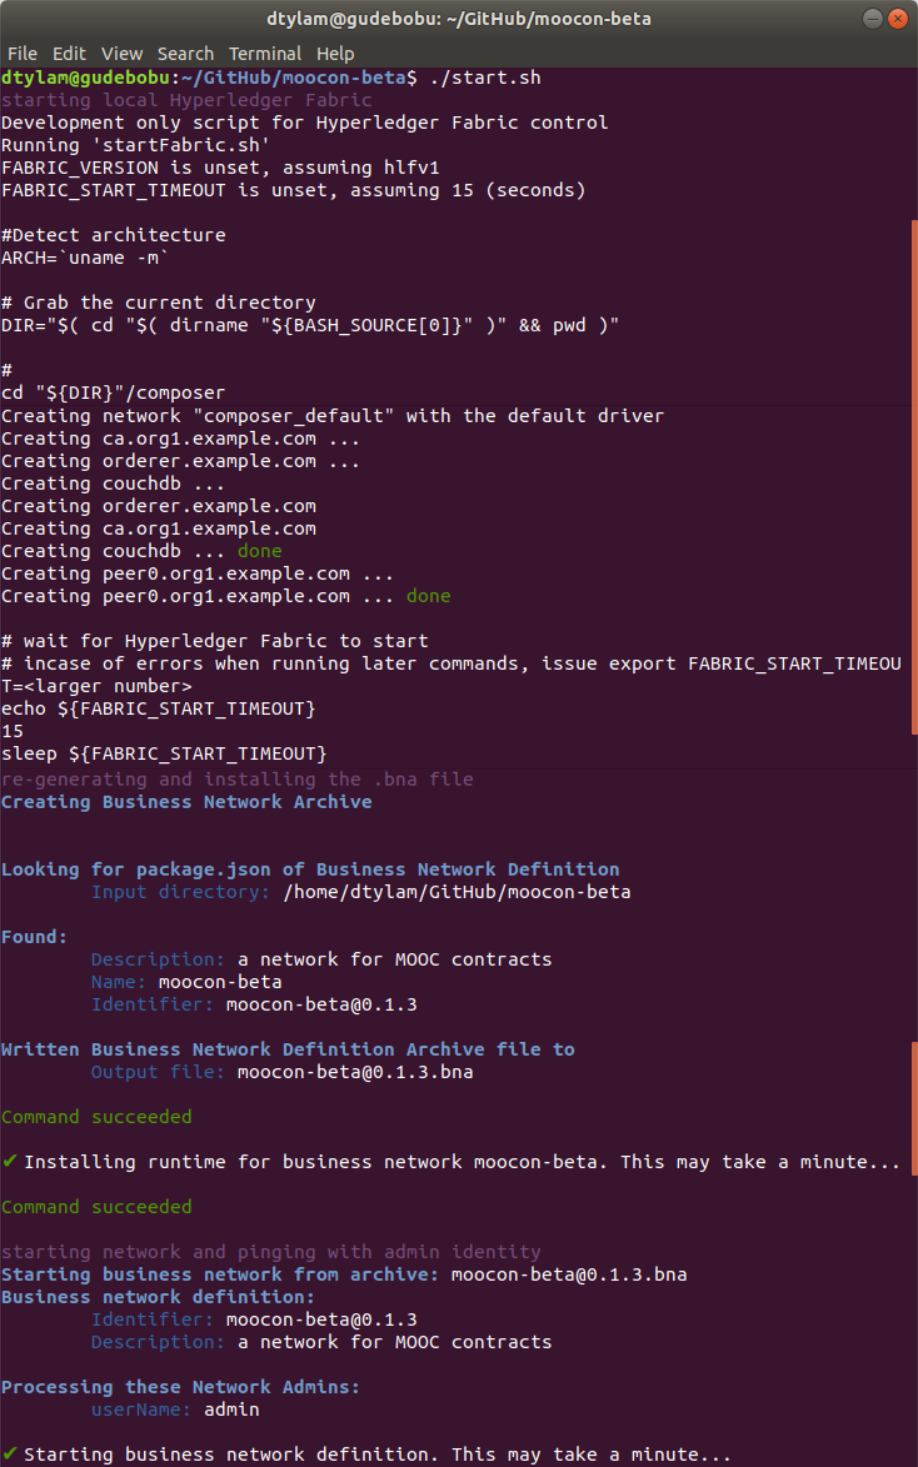
\includegraphics[width=0.9\textwidth]{startsh}
        \caption[Blockchain Startup Script Screenshot]
            {Screenshot of the start.sh script in action in a command line interface}
        \label{fig:startsh}
    \end{figure}
    \item \textit{load\_participant.sh}: this script connects as the blockchain administrator and creates 
    three \textit{Learner}, four \textit{Teacher} and two \textit{Reader} participants on the blockchain.
    \begin{figure}[!ht] 
        \centering    
        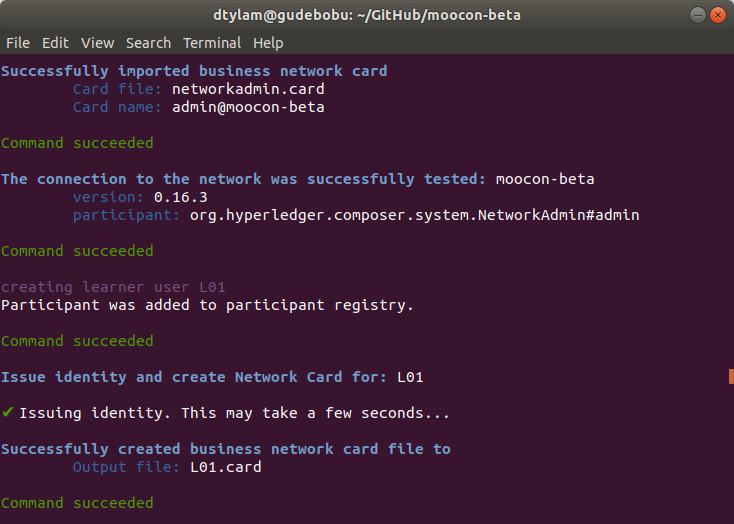
\includegraphics[width=0.9\textwidth]{load_participantsh}
        \caption[Participant Loading Script Screenshot]
            {Screenshot of the load\_participant.sh script in action in a command line interface}
        \label{fig:load_participantsh}
    \end{figure}
    \item \textit{destroy.sh}
    \begin{figure}[!ht] 
        \centering    
        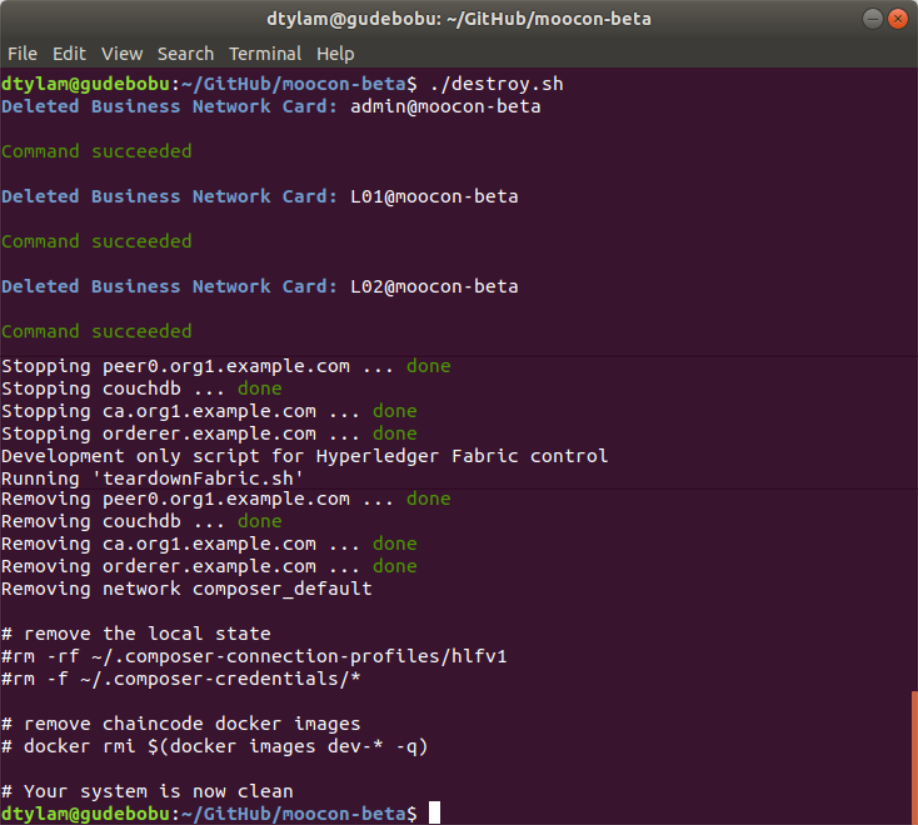
\includegraphics[width=0.9\textwidth]{destroysh}
        \caption[Blockchain Teardown Script Screenshot]
            {Screenshot of the destroy.sh script in action in a command line interface}
        \label{fig:destroysh}
    \end{figure}
\end{enumerate}

The GitHub repository used is hosted at \href{https://github.com/dtylam/moocon-beta}{\underline{github.com/dtylam/moocon-beta}}.
Three branches (significant iterations) were created for this component, below in chronological order:
\begin{enumerate}
	\setlength\itemsep{0em}
    \item \textit{moocon-alpha}: 
    \item \textit{master}
    \item \textit{bcu}
\end{enumerate}

\subsection{Application Program Interface}

Loopback

multiuser authentication

\section{Automatic Marking Service Development}

\section{Client Applications Development}

\subsection{Learner Application}
Component driven development

\subsection{Teacher Application}


\section{Test Driven Development}

mocha

postman
